\documentclass[french]{beamer}

\usetheme{metropolis}
\usecolortheme{metropolis}
\uselanguage{French}
\languagepath{French}
\usepackage[utf8]{inputenc}
\usepackage[T1]{fontenc}
\usepackage{babel}

\usepackage{pgfpages}
\setbeameroption{show notes on second screen=bottom}

\usepackage[sfdefault]{FiraSans}
\usepackage{scrextend}
\usepackage{eqnarray,amsmath}
\usepackage{tikz}
\definecolor{mygrey}{RGB}{35, 55, 59}
\definecolor{mygreen}{RGB}{39, 174, 96}
\definecolor{myblue}{RGB}{41, 128, 185}
\definecolor{mypurple}{RGB}{142, 68, 173}
\definecolor{fgreen}{RGB}{184, 233, 148}
\definecolor{fred}{RGB}{248, 194, 145}
\definecolor{fblue}{RGB}{130, 204, 221}

\title{[4.1] Middleware : Voiture autonome}
\date{~~~24~~Avril~~2020~~~}
\author{Quentin BRATEAU}
\institute{\vspace{-0.25cm}\hspace{-0.2cm}
\includegraphics[width=3.1cm]{logo.jpg}}


\begin{document}
    \maketitle
    \changefontsizes{10pt}

    \addtobeamertemplate{frametitle}{}{%
    \begin{tikzpicture}[remember picture,overlay]
    \node[anchor=south west] at (current page.south west) {
\includegraphics[height=0.7cm]{logo.jpg}};
    \end{tikzpicture}}
    \setbeamerfont{caption}{size=\footnotesize}

    \begin{frame}{Objectif \& Exigences}
        \begin{columns}
            \begin{column}{0.42\textwidth}
                \begin{figure}
                    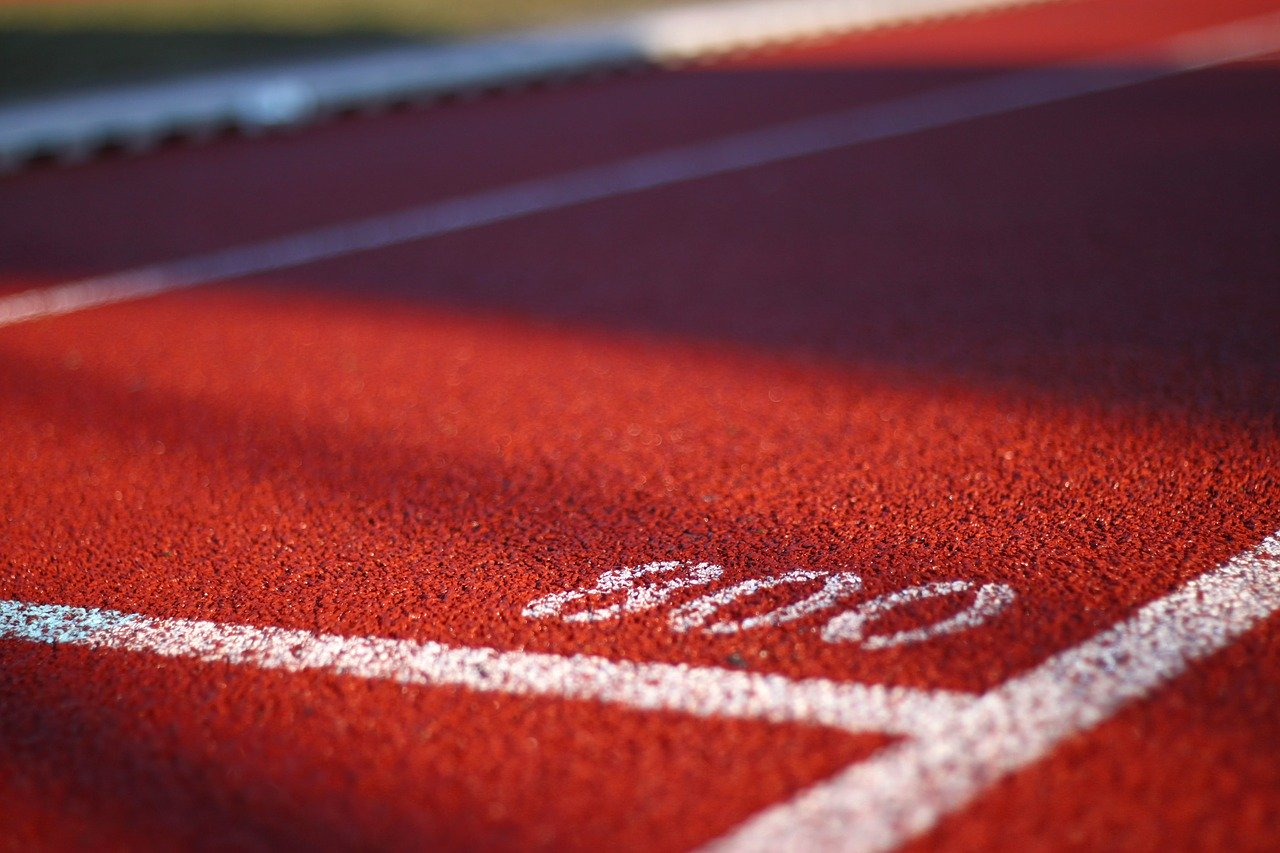
\includegraphics[width=\textwidth]{Images/piste.jpg}
                    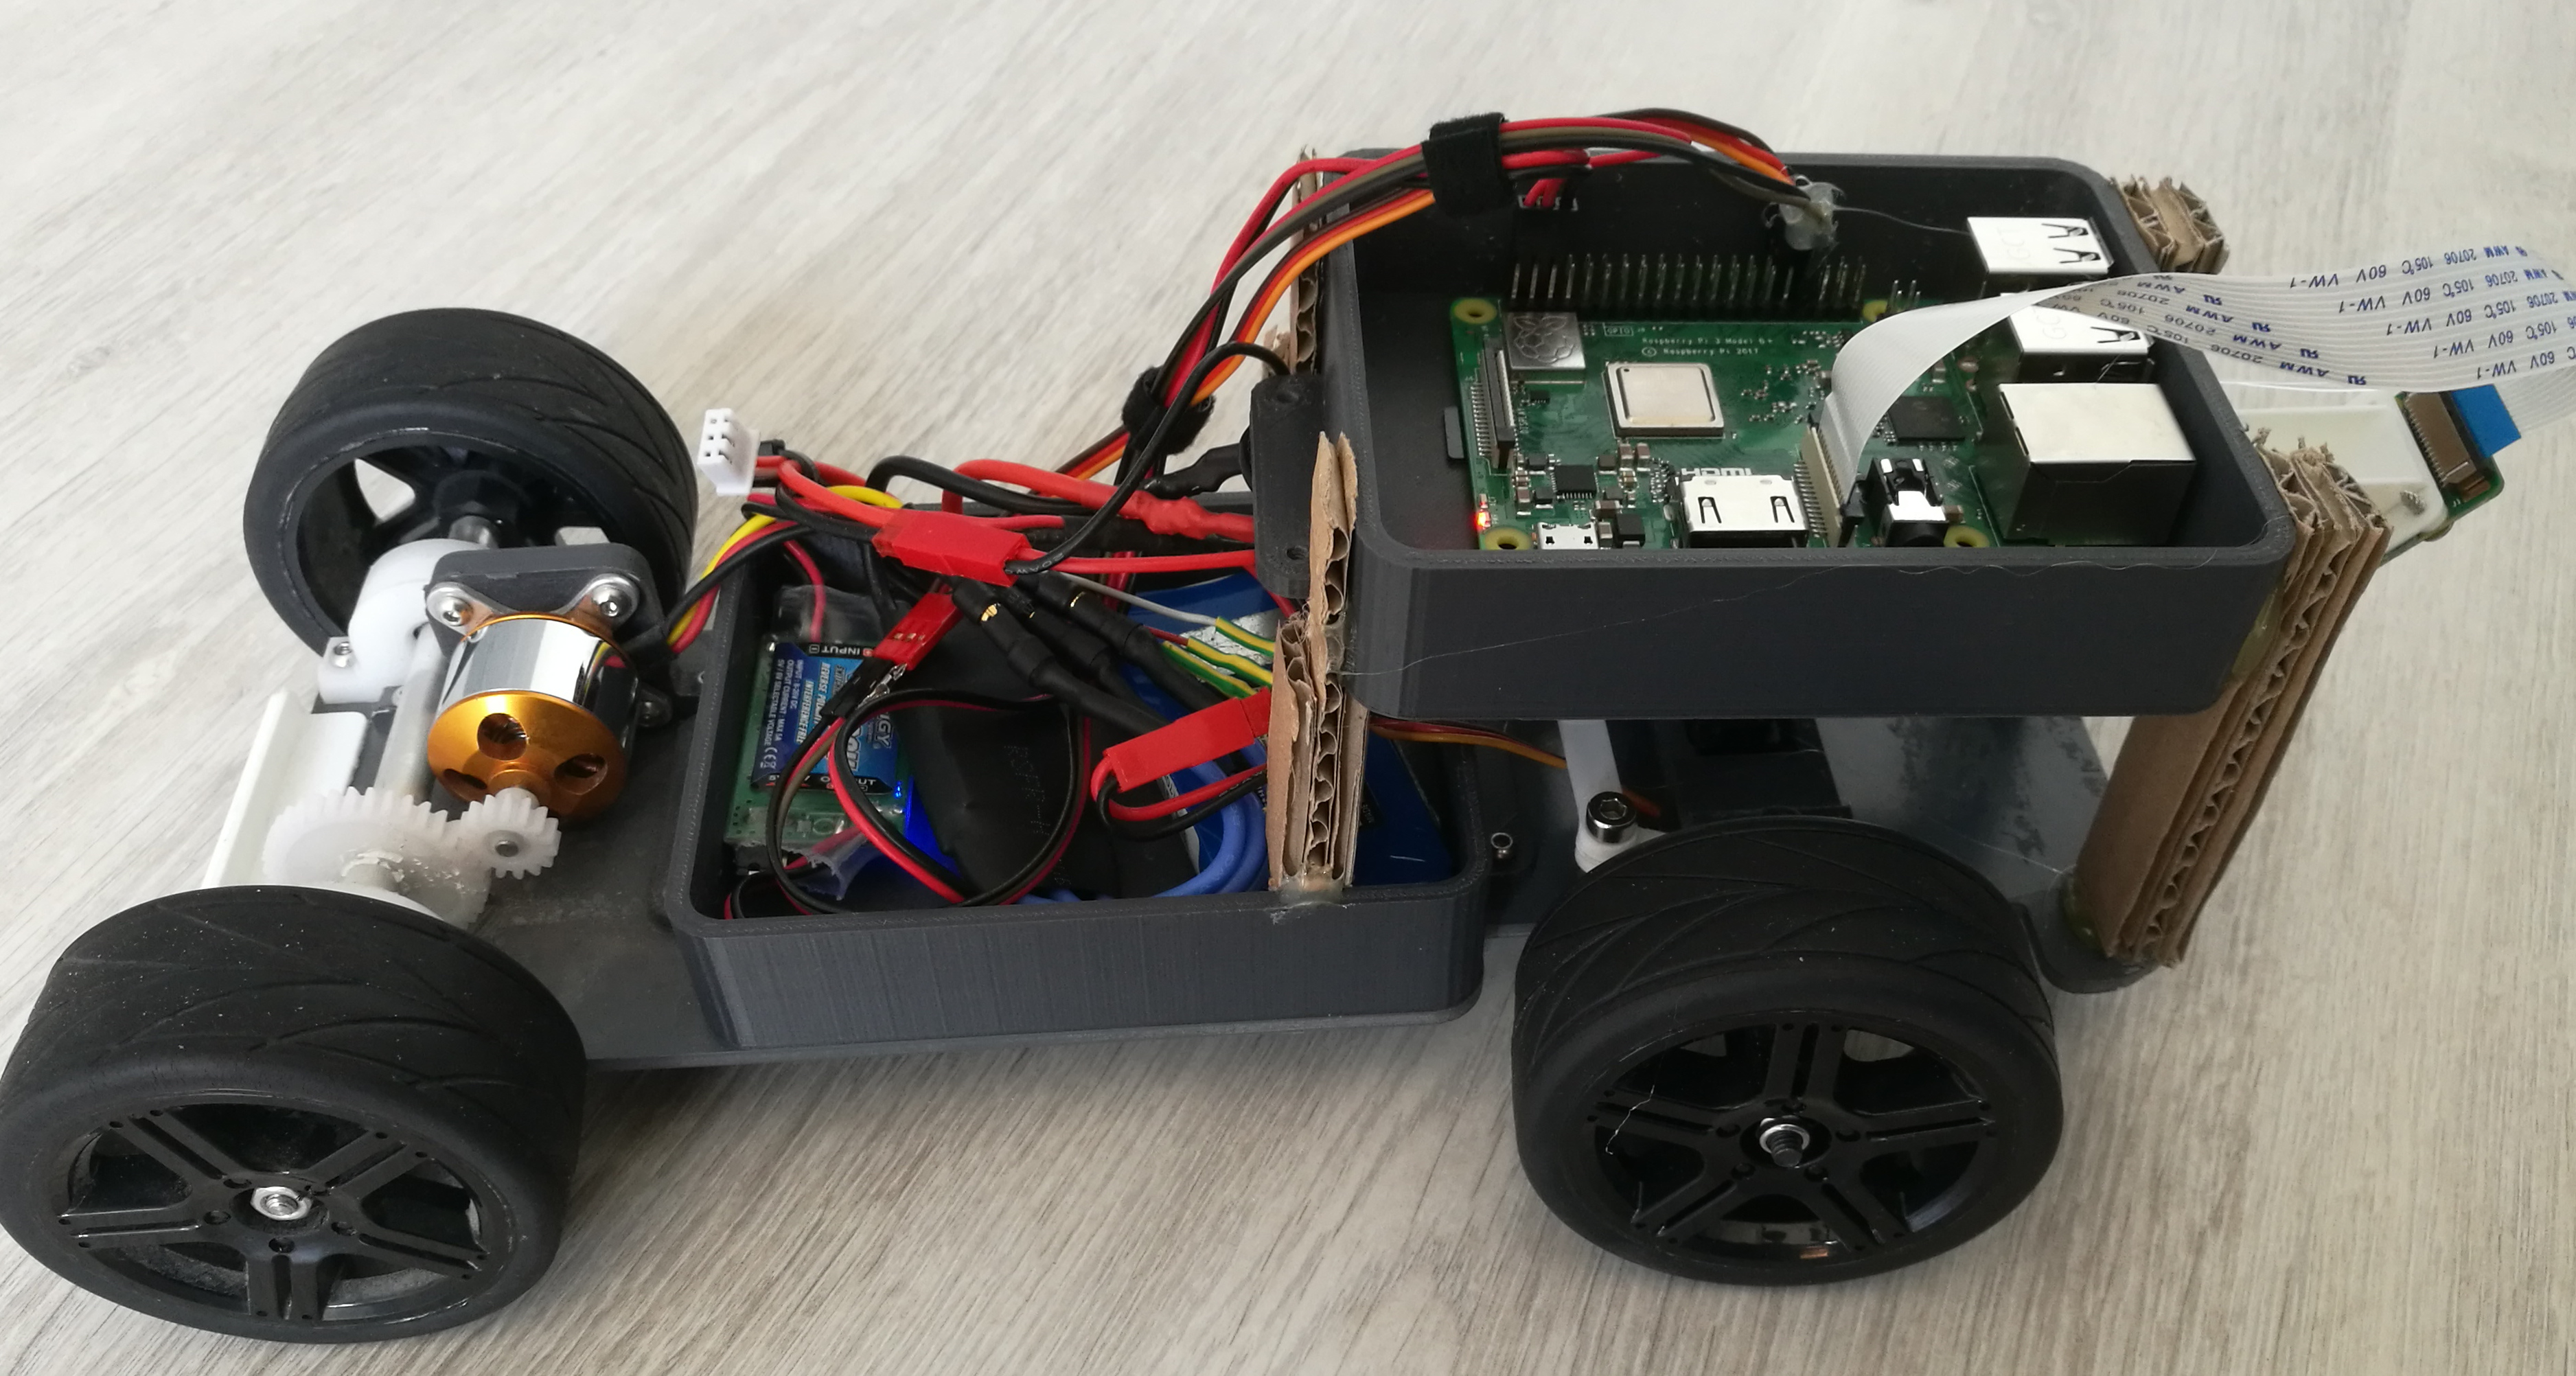
\includegraphics[width=\textwidth]{Images/kart.jpg}
                    \caption{Système actuel}
                \end{figure}
            \end{column}

            \begin{column}{0.54\textwidth}
                \textbf{Objectifs du système}
                \begin{itemize}
                    \item Autonomie
                    \item Rapidité
                    \item Suivi de ligne
                \end{itemize}
                \vspace{0.5cm}
                \textbf{Exigences}
                \begin{itemize}
                    \item Tour de piste
                    \item Vitesse minimum $3\ m.s^{-1}$
                    \item Connaitre sa position
                \end{itemize}
            \end{column}
        \end{columns}

        \note{
            \textbf{Time code} : 4:50 $\rightarrow$ 4:20 \\
            \vspace{0.5cm}
            Objectif automatiser voiture construite Atelier CNC \\
            Réaliser Autonomie tour de piste athlétisme + rapidement possible \\
            Startégie : Suivi d'une ligne de piste \\
            \vspace{0.5cm}
            Présenter principales exigences système \\
            Tour de piste peu importe la géométrie de celle-ci
        }
    \end{frame}

    \begin{frame}{Architecture logicielle}
        \begin{figure}
            \resizebox{\textwidth}{!}{
            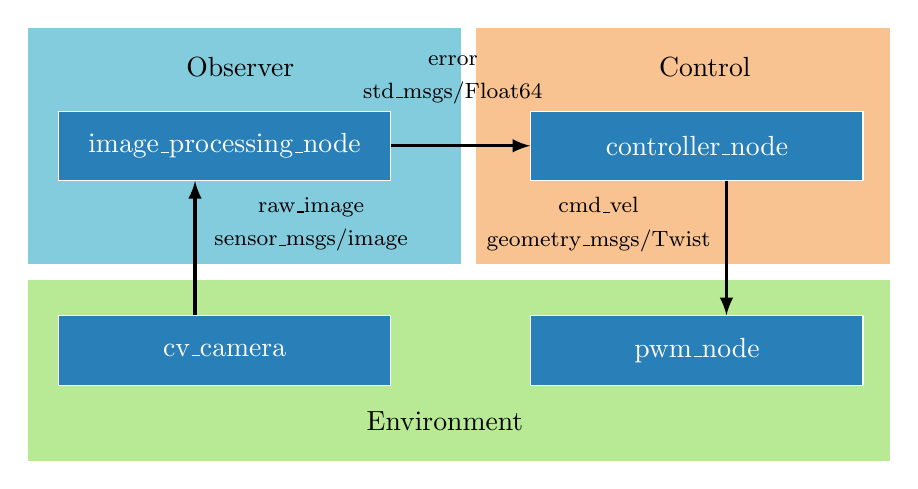
\begin{tikzpicture}
                \fill [fgreen] (-2.5,-1.5) rectangle (8.45,0.8);
                \fill [fblue] (-2.5,1) rectangle (3,4);
                \fill [fred] (3.2,1) rectangle (8.45,4);

                \node[] at (2.8,-1) {Environment};
                \node[] at (0.2,3.5) {Observer};
                \node[] at (6.1,3.5) {Control};
                \node[text width=3.8cm, align=center] at (1.1,1.5) {\footnotesize raw\_image \\ sensor\_msgs/image};
                \node[text width=3.8cm, align=center] at (2.9,3.34) {\footnotesize error \\ std\_msgs/Float64};
                \node[text width=3.8cm, align=center] at (4.75,1.5) {\footnotesize cmd\_vel \\ geometry\_msgs/Twist};

                \tikzstyle{box}=[rectangle, draw, minimum width=12em, minimum height=2.5em, text centered, color=white]
                \node[box, fill=myblue] (C1) at (0,-0.1) {cv\_camera};
                \node[box, fill=myblue] (C2) at (0,2.5) {image\_processing\_node};
                \node[box, fill=myblue] (C3) at (6,2.5) {controller\_node};
                \node[box, fill=myblue] (C4) at (6,-0.1) {pwm\_node};

                \tikzstyle{bind}=[->,very thick,>=latex]

                \draw[bind] (C1.130) to (C2.230);
                \draw[bind] (C2) to (C3);
                \draw[bind] (C3.310) to (C4.50);
            \end{tikzpicture}}
            \caption{Architecture logicielle}
        \end{figure}

        \note{
            \textbf{Time code} : 4:20 $\rightarrow$ 3:45 \\
            \vspace{0.5cm}
            Architecture classique avec ROS \\
            Partie Environnement, Controle, Commande \\
            \vspace{0.5cm}
            Acquérir image piste node \textit{cv\_camera}\\
            Traitement d'image node \textit{image\_processing\_node} \\
            Elaboration loi commande \textit{controller\_node} \\
            Commande actionneurs \textit{pwm\_node} \\
            \vspace{0.5cm}
            Bouclage complet pour notre architecture logicielle
        }
    \end{frame}

    \begin{frame}{Architecture matérielle}
        \begin{figure}
            \centering
            \resizebox{\columnwidth}{!}{
            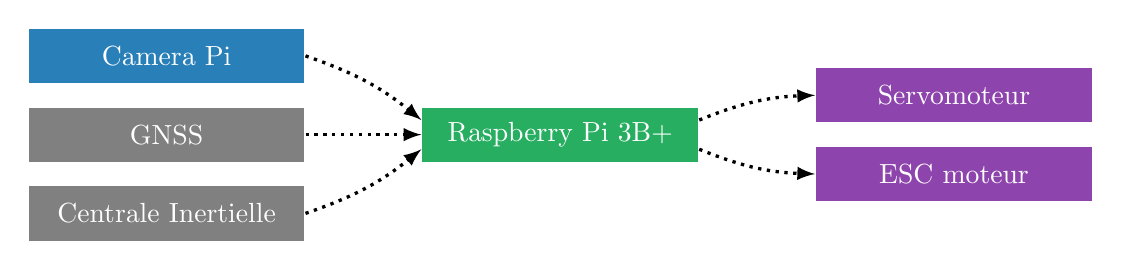
\begin{tikzpicture}
                \tikzstyle{box}=[rectangle, draw, minimum width=10em, minimum height=2em, text centered, color=white]
                \node[box, fill=myblue] (C1) at (0,1) {Camera Pi};
                \node[box, fill=gray] (C2) at (0,0) {GNSS};
                \node[box, fill=gray] (C3) at (0,-1) {Centrale Inertielle};
                \node[box, fill=mygreen] (B) at (5,0) {Raspberry Pi 3B+};
                \node[box, fill=mypurple] (A1) at (10,0.5) {Servomoteur};
                \node[box, fill=mypurple] (A2) at (10,-0.5) {ESC moteur};

                \tikzstyle{bind}=[->,dotted,very thick,>=latex]

                \draw[bind] (C1.east) to[bend left=10] (B.174);
                \draw[bind] (C2.east) to (B);
                \draw[bind] (C3.east) to[bend right=10] (B.186);
                \draw[bind] (B.6) to[bend left=10] (A1.west);
                \draw[bind] (B.-6) to[bend right=10] (A2.west);
            \end{tikzpicture}}
            \caption{Diagramme de l'architecture matérielle}
        \end{figure}
        
        \note{
            \textbf{Time code} : 3:45 $\rightarrow$ 3:00 \\
            \vspace{0.5cm}
            3 Parties : Capteur, Traitement, Actionneurs \\
            \vspace{0.5cm}
            \textbf{Capteur} \\
            3 Capteurs à disposition :
            Ne se sert que caméra \\
            \vspace{0.5cm}
            \textbf{Traitement} \\
            Gérée Raspberry Pi 3B+ \\
            \vspace{0.5cm}
            \textbf{Actionneurs} \\
            Servomoteur pour direction avant \\
            ESC controller moteur arrière donc vitesse voiture \\
            \vspace{0.5cm}
            Commande actionneurs gérée par PWM hardware du RPI
        }
    \end{frame}

    \begin{frame}{Traitement d'image}
        \begin{columns}
            \begin{column}{0.44\textwidth}
                \textbf{N\oe ud ROS}
                \begin{itemize}
                    \item OpenCV 4.0
                    \item Driver \textit{cv\_camera}
                    \item erreur $e = e_x + e_y$
                \end{itemize}
                
                \begin{figure}
                    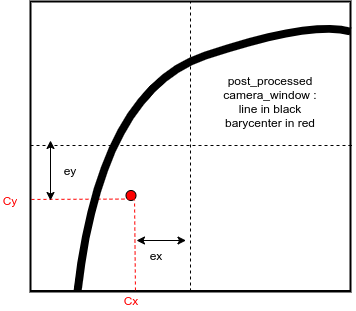
\includegraphics[width=0.5\textwidth]{Images/ip.png}
                    \caption{Calcul de l'erreur}
                \end{figure}
            \end{column}
            \begin{column}{0.55\textwidth}
                \begin{figure}
                    \centering
                    \resizebox{\textwidth}{!}{
                    \begin{tikzpicture}
                        \tikzstyle{box}=[rectangle, draw, minimum width=12em, minimum height=2em, text centered, color=white, fill=myblue]
                        \node[box] (T0) at (0,4.8) {Flou Gaussien};
                        \node[box] (T1) at (0,3.6) {Binarisation};
                        \node[box] (T2) at (0,2.4) {Dilatation};
                        \node[box] (T3) at (0,1.2) {Erosion};
                        \node[box] (T4) at (0,0) {Contours avec stats};
        
                        \node (ini) at (5, 4.8) {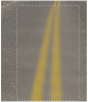
\includegraphics[height=1.2cm]{Images/initial.png}};
                        \node (bin) at (5, 3.6) {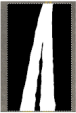
\includegraphics[height=1.2cm]{Images/binarize.png}};
                        \node (dil) at (5, 2.4) {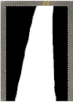
\includegraphics[height=1.2cm]{Images/dilate.png}};
                        \node (ero) at (5, 1.2) {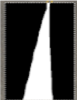
\includegraphics[height=1.2cm]{Images/erode.png}};
                        \node (con) at (5, 0) {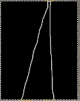
\includegraphics[height=1.2cm]{Images/contour.png}};
        
                        \tikzstyle{bind}=[->,very thick,>=latex]
                        \tikzstyle{dot}=[->,loosely dotted,very thick,>=latex]
        
                        \draw[bind] (T0) to (T1);
                        \draw[bind] (T1) to (T2);
                        \draw[bind] (T2) to (T3);
                        \draw[bind] (T3) to (T4);
        
                        \draw[dot] (T0) to (ini);
                        \draw[dot] (T1) to (bin);
                        \draw[dot] (T2) to (dil);
                        \draw[dot] (T3) to (ero);
                        \draw[dot] (T4) to (con);
                    \end{tikzpicture}}
                    \caption{Chaine de traitement d'images}
                \end{figure}
            \end{column}
        \end{columns}

        \note{
            \textbf{Time code} : 3:00 $\rightarrow$ 2:00 \\
            \vspace{0.5cm}
            Implémenté node de traitement images \\
            Basé sur lib traitement image Opencv4.0 \\
            Récupère image \textit{cv\_camera}, node de communauté ROS\\
            Calculer erreur à partir de différence centre image/barycentre ligne \\
            Erreur totale = somme des erreurs suivant 2 axes de l'image \\
            \vspace{0.5cm}
            \textbf{Flou Gaussien} Nettoyer image bruit \\
            \textbf{Binarisation} Détacher ligne du fond de l'image \\
            \textbf{Dilatation/Erosion} Refermer ligne + supprimer erreurs binarisation
            \textbf{Contours avec stats} Obtenir le barycentre de ligne\\

            \vspace{0.5cm}
            Commande actionneurs gérée par PWM hardware du RPI
        }
    \end{frame}

    \begin{frame}{Simulation}
        \begin{columns}
            \begin{column}{0.5\textwidth}
                \vspace{0.3cm}
                \textbf{Avantage ROS}
                \begin{itemize}
                    \item Réel $\hookrightarrow$ Simulé
                    \item Même topics
                    \item Test des autres n\oe uds
                \end{itemize}
                \textbf{V-REP} \\ Modélisation en 3 couches
                \begin{itemize}
                    \item Inertielle
                    \item Collisions
                    \item Design
                \end{itemize}
            \end{column}

            \begin{column}{0.5\textwidth}
                \centering
                \begin{figure}
                    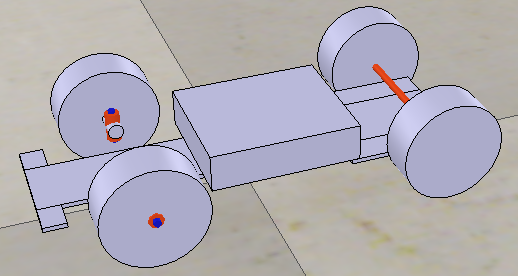
\includegraphics[width=\textwidth]{Images/collide.png}
                    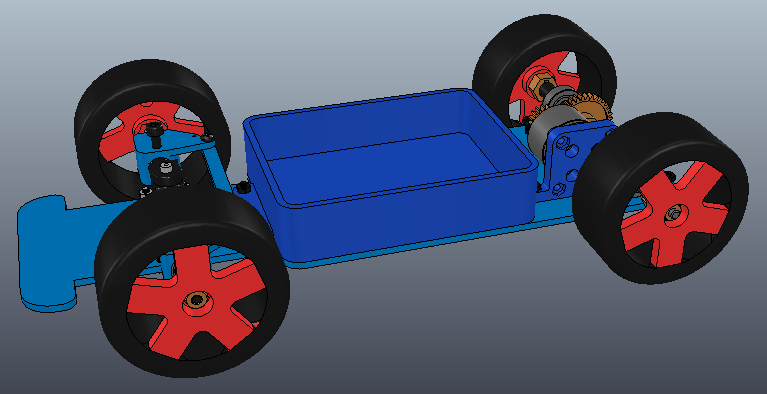
\includegraphics[width=\textwidth]{Images/real.png}
                    \caption{Modélisation dans V-REP}
                \end{figure}
            \end{column}
        \end{columns}

        \note{
            \textbf{Time code} : 2:00 $\rightarrow$ 1:15 \\
            \vspace{0.5cm}
            \textbf{Avantage ROS} $\dots$\\
            \vspace{0.2cm}
            Utiliser Simulateur V-REP \\
            Interfaceable avec ROS via script en LUA \\
            Modélisation 3 couches : \\
            \vspace{0.2cm}
            \textbf{Partie Calculs} : Inertielle + Collision \\
            Modélisée par pavés droits et cylindre \\
            Simplifier grandement calculs $\rightarrow$ Simu + fluide \\
            Masquée affichage par suite \\
            Permet définir comportement voiture

            \vspace{0.2cm}
            \textbf{Partie Affichage} : Design \\
            Import des fichier CAO sous forme Mesh \\
            Permet affichage esthétique voiture \\
        }
    \end{frame}

    \begin{frame}{Résultats \& Conclusion}
        \vspace{0.8cm}
        \begin{columns}[c]
            \begin{column}{0.50\textwidth}
                \centering
                \textbf{Système Réel}
                \begin{itemize}
                    \item Boucle caméra fonctionnelle
                    \item Manque d'outils
                    \item Manque de matériel
                \end{itemize}
            \end{column}
            \vrule{}
            \begin{column}{0.50\textwidth}
                \centering
                \textbf{Système Simulé}
                \begin{itemize}
                    \item Parfaitement fonctionnel
                    \item Vitesse atteinte $6~m.s^{-1}$
                    \item Conditions optimales
                \end{itemize}
            \end{column}
        \end{columns}
        \vspace{0.5cm}

        \textbf{Projet}
        \vspace{-0.3cm}
        \begin{itemize}
            \item Architecture ROS sur système réel
            \item Développement avec GitHub
            \item Méthode AGILE adaptée à structure ROS
        \end{itemize}

        \note{
            \textbf{Time code} : 1:15 $\rightarrow$ 0:00 \\
            \vspace{0.5cm}
            \textbf{Système réel} \\
            Boucle Caméra fonctionnelle mais pas testée en conditions réelles \\
            Manque outils : Imprimante 3D $\rightarrow$ support camera \\
            Manque matériel : GPS et Centrale inertielle \\
            \vspace{0.5cm}
            \textbf{Système simulé} $\dots$ \\
            \vspace{0.5cm}
            \textbf{Projet en général} $\dots$
        }
    \end{frame}

    \maketitle
\end{document}